% Chapter 2

\chapter{Introduction} % Main chapter title

\label{Chapter2} % For referencing the chapter elsewhere, use \ref{Chapter1} 

\section{Background and Problem Statement}
The biomechanical characterization of soft tissues has gained attention
in medical research, in areas such as medical image analysis and visualization.
For many years, the obtained medical diagnoses were often based on the assumptions of experts or 
their accumulated experience. While this information have proven to be useful in general, 
these methods have limitations in cases where quantifiable data is necessary, specifically for computer-assisted systems, e.g,
medical diagnosis, therapy, and training \cite{Kauer2002}.
To gather the material data, e.g., elasticity, stiffness, response under deformation and temperature, it is required 
to gain access to the soft tissues and perform in-vivo testing experiments. 
However, obtaining accurate biomechanical data can be challenging
due to the invasive nature of the procedures and the difficulty in maintaining constant and reproducible internal or external factors  
in experimental configurations.\\

%Precise knowledge about the biomechanical characterization of soft tissues has received attention
%in medical research, e.g., medical image analysis and visualization.
%For many years, the obtained medical diagnosis have come from assumptions of experts or 
%accumulated experience. This information, although proven to be useful, has its limitations 
%when computed-assisted systems like, medical diagnosis, therapy, and training, rely on 
%more quantifiable data \cite{Kauer2002}. To gather this data, it is important to gain access
%to the tissues and perform in-vivo testing experiments. For organs, this procedure is nearly 
%impossible to achieve, due to the involvement of an invasive procedure, and the lack of constant
%and reproducible external and internal factors. \\ 
Especially, when it comes to internal organs, obtaining reliable data for examination after their 
extraction is difficult because the material properties can vary between samples or testing 
locations on the same organ. This is due to the influence of various factors such as changes in blood pressure, changes in material properties 
over time, symptoms of disease, and more. In addition, another problem is the lack 
of replication, due to the use of different individuals' organs, which introduces more external
factors into the equation. Moreover, given a tissue sample, it is difficult to properly 
characterize the material due to its anisotropic property, which can lead potentially
 to inaccuracies in the result.

%Particularly in the case of internal organs, one of the challenges associated with their extraction 
%is that some material properties may change despite examination of the same sample. Their biomechanical properties 
%depend on other factors, such as changes in blood pressure, changes in material properties 
%over time, symptoms of disease, and more. In addition, another problem is the lack 
%of replication, due to the use of different individuals' organs, which introduces more external
% factors into the equation. Moreover, given a tissue sample, it is difficult to properly 
% characterize the material due to its anisotropic property, which can lead to inaccuracies in the result.\\

In the situation where the material data can be collected in a constant, fast and reliable
process, a material model can be established and the computer-aided systems can predict 
the mechanical behavior of soft tissues, providing preoperative calculations. 
This demonstrates the importance of material data collection and material model development, 
especially in the context of computational models such as engineering simulation models created finite 
element analysis (FEA) software and their medical applications in medical devices, surgical 
procedures, and training softwares. By using accurate material models, the accuracy of the simulation 
can be improved, aiding in a better understanding and predicting a soft tissue response 
to external stimuli, making them more useful in medical research and other related applications.\\

\section{Objective and Scope of the Study} 

Soft materials often exhibit nonlinearity, making the finite element method (FEM) a common approach 
for their analysis and solving continuum mechanical problems. 
Although FEM facilitates the analysis of complex structures with complex material 
behavior, simulating such materials requires high computational costs.\\

The main objective of this study is to identify the key parameters of soft materials and their 
influence on the development of a material model based on inverse finite element method (iFEM) approach. 
By identifying these key parameters, an attempt is made to approximate the behavior of 
complex materials through a simplified material model and
assess its potential future applications in medical research and its use with organs.\\

To achieve this goal, an experimental configuration will be selected, and a computational model will be 
developed to use an iFEM approach to identify the key material parameters of the given soft material. 
With this method, it was possible to match the results of the computational model to the experimental 
data, and validate the model with additional data points. 

This study aims to establish a framwork for identifying the key parameters of any soft material, providing 
faster results for future experiments or use cases. By contibuting to this framework, it will be 
possible to accelerate the development of material models for practical applications in medical research and development.

%----------------------------------------------------------------------------------
\section{State of the Art}

\subsection{Experimental Characterization for Soft Materials}
%material testing
In order to characterize the mechanical behavior of a test specimen, the most common method
method is to mechanically load the specimen and measure the response of the force against 
the displacement \cite{Bergström2015}. 

%Soft materials challenges in experimental deign


- Soft synthetics materials like soft gels are one example for soft synthetic materials. These
are commomly applied for tissue engineering applications. Nevertheless, due to their elastic 
modulus range (kPa) present some challenges for the design of experimental testing \cite{Liu2009}.

\subsubsection*{Uniaxial Tension/Compression Testing}

This is one of the most common using methods to determine an stress-strain relationship.
For uniaxial tension cases, the specimen is well loaded in a machine by gripping the ends and perfoming 
tension tests. Then, the deformation is usually measured with a strain gauge. \cite{Bergström2015}

As for compression test, the specimen is loaded by placing it inbetween from two plates 
and compressing the material. \cite{Bergström2015}

This method allows the validation of several computational models as it provides with
 searched parameters done with other experimental procedure. 



\subsubsection*{Aspiration Experiment}

Tissue aspiration experiments introduces an aspiration tube which is put against the 
soft tissue, generating a vacuum. An advantageous feature of this experiment is that 
it can be perfomed in-vivo and ex-vivo.
With the help of a mirror placed next to aspiration 
hole, the reflection of the side-view of the tissue can be captured with a video camera.
This camera captures the images of the iluminated surface of the material and the 
aspiration pressure is captured through a sensor. Through this process the captured 
profile of the tissue is obtained and this can be used to characterize the deformation 
and analyze the viscoelastic properties of the soft tissue\cite{Kauer2002}.

\subsubsection*{Indentation}
Indentation have being gaining popularity in the last decades and it is now one of
 the most spread experiments for material parameter identification.
 Indentation presents a bigger advantage in cases where it is not possible to load
 test specimens in a more conventional way.\cite{Bergström2015} As some materials, e.g. biomaterials do not always 
 allow the use of uniaxial or biaxial tensile testing, the
 use of identation testing is essential.  

Indentation possesses advantageous characteristics for the mechanical characterization
of soft materials. \cite{Liu2009}
Nanoindentation or microindentation it is useful for the evaluation of
nonlinear viscoplastic responses. \cite{Bergström2015}

The indentation testing set up is described as followed: As shown in Fig. \ref{fig:Nanoindentation} 
A system applies a certain force to an attached indenter rod where and specific 
indenter tip. After the indenter tip goes to a determined displacement, 
it is possible to obtain a Load-displacement curve.
The deformation can be measured through an capacitance gauge \cite{Bergström2015}
or also optically (via laser measurements).

 \begin{figure}[th]
        \centering
        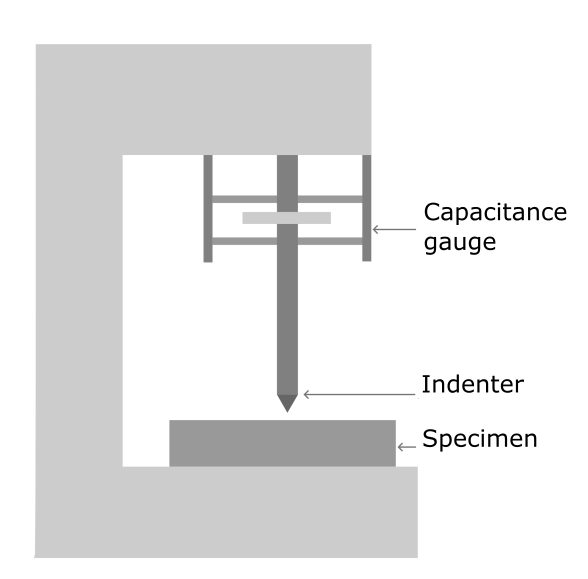
\includegraphics[width=8cm]{Images/nanoindentationbigletter}
        \decoRule
        \caption[Nanoindentation]{Nanoindentation experiment setup.}
        \label{fig:Nanoindentation}
        \end{figure}


-identation in materials
- Identation in soft materials (organs)
- Why is identation relevant in organs
-what advantages and disadvantges does identation provides
-why is relevant for this project 

%---------------------------------------------------------------------------------
\subsection{Material Modeling of Soft Materials}
 
Relevant papers tends to use hyperelastic models to represent soft materials as the viscoelasticity 
is usually neglected. 
% why do they use hyperelastic formulas? Why is it possible to neglect the viscoelasticity
%Revisar
Material model are very relevant for the simulation model (Kauer2002).
Soft tissues are approximated as near incompressible due to their highly water content.  
%viscoelastic example
For the aspiration experiment conducted by Kauer they used the following strain energy
function based on the model of Susanne and Bathe (SusanneandBAthe1987)
%Revisar


As derivative from this formula for the uteri metrial modeling the formula used was:

%---------------------------------------------------------------------------------
\subsection{Inverse Finite Element Method for Parameter Identification}

An inverse finite element (FE) approach requires usually a certain experimental model,
 which generates certain information e. g. load-displacement curve, and through 
a verified computational model match the given data curve to obtain further information 
of the material's behavior e. g., stress-strain curve.

Specially for nonlinear cases \cite{Husain2004}, where the complexity of the problems 
increases, and the interest is focused to generate an action which results in a 
certain output response, is where an inverse finite element approach can be helpful 
to discover a certain variable going from an ouput data. Through an iterative process it is 
possible to describe the material's behavior and validate the output data it 
through other established testing e. g., uniaxial testing.

Though this approach does not always give a hundred percent match in all obtain points 
or zones, it allows the researcher to understand the influences of certain parameters 
for the materials. This is specially useful for complex materials as biomaterials. 

Biomaterials, as mentioned previously, depends on multiple external factors, e.g., blood 
pressure, affected diseases and the their material properties is constantly changing. 
This issue does not allow the researcher to develop a proper material model which is 
usable for multiple use-cases. 

Therefore, the importance of the inverse element method as relevant key for estimating 
constantly changing parameters in soft materials.

For biomechanical models, where the models require knowledge from local properties \cite{Chai2013},
as the biomaterial is not isotropic; it is possible to identify a parameter e.g. Young's Modulus 
from a 3D model. The model can be matched to multiple experiments and multiple samples in different areas,
which allows a better representation of the material for further analysis.

The inverse FE approach can used by optimizing the searched parameter by matching the simulated data
to a section of a experimental curve and extending this process through some iterations. 
Nevertheless, it is important to clarify that this method also requires making assumptions to some values.
Furthermore, it is relevant to document these assumptions for the further analysis. 
With the combination of assumptions, experimental data, and a optimized and matched simulation curve, it
is possible to solve the complexity of biomechanical models.
 
In next sections some of the experimental models and the material models for bio and soft materials are 
going to be explained to get a further understanding in how is possible to get a realiable computational 
model for further reasearch

\subsubsection*{Synthetic Soft Materials}

Synthetics materials are commonly used to validate an inverse parameter identification process. 
Usually these synthetic, soft materials provide similar mechanical behavior to it's biomaterials 
counterparts. This characterization allows to validate a proposed inverse finite element approach process
before its applicatoin with a biomaterial, where the measurements to gather the experimental data are 
some in-vivo, and more challenging to recreate.


For example, Silgel, a very soft gel-like material \cite{Kauer2002} was used for the experimental 
validation of the inverse finite element method proposed, to characterized the tissue of 
a human uteri. In this work, the tensile behavior of the material was predicted through the 
parameters obtained in the aspiration method. The matching procedure is optimize through 
an objective function, which consists of the squared differences between the simulation 
and exprimental data. With an optimization algorithm an optimal set of the following parameters 
was found: the material parameters \(\mu_i\) [N/m\textsuperscript{2}] and the bulk Modulus
\(\kappa\) [N/m\textsuperscript{2}]. This method showed good prediction quality of the mentioned 
material parameters.

\subsubsection*{Biomaterials}
Biomaterials as mentioned before, represent a challenge due its difficult access and lesser replicability.
Therefore these materials are usually used for the experimetnal validation of a methd applied previously in 
synthetic materials. 
 Following the first example of the Silgel in the previous section, the inverse finite element parameter
 estimation is applied now on human uteri \cite{Kauer2002} through in vivo and ex vivo measurements of the human tissue of 
 different patients. It was mentioned, that in comparison from the silgel the uterus possesses a complex 
 multi layered structure with strongly anistropic and viscoelastic properties. Nevertheless, five 
 material parameters were determined, based on the strain energy function to model a human uterus (Yamada 1970).
Through the same inverse method applied with the synthetic material, the obtained parameters facilitated the prediction of stress-elongation curves for tensile experiments. The 
 resulting curves showed the difference of stiffness for in vivo and ex vivo measurements and the material 
 singurality for each uterus.


\subsection{Standard Verification and Validation for Computational Solid Mechanics (ASME)}
\subsubsection*{VV40}


%---------------------------------------------------------------------------------

\section{Overview}